\chapter{Introduction, apprentissage supervisé, bornes de généralisation}

\myminitoc

\sect{Introduction}

\paragraph{Qu'est ce que le machine learning ?}
Le machine learning est le développement d'algorithmes qui apprennent tout seul à partir de données. On distingue deux catégorie :
\begin{itemize}
	\item L'apprentissage supervisé : qui apprend avec des données étiquetées afin de faire de la classification, de la régression ou encore de la hiérarchisation.
	\item  L'apprentissage non supervisé : qui trouve la structure d'un jeu de données afin de faire du clustering ou de la réduction de dimensions.
\end{itemize}
Les applications principales du machine learning sont alors la vision par ordinateur, la robotique, la reconnaissance vocale, le traitement du langage, etc ...

\sect{Apprentissage supervisé}

\DEF{
	Dans la suite on utilisera les notations suivantes :
	\begin{itemize}
		\item On pose $\bm{S = \{ z_i = (x_i, y_i) \}_{i = 1}^m}$ un ensemble de $\bm{m}$ exemples d'entraînement indépendants et identiquement distribués selon une une distribution inconnue $\bm{\dist}$ sur l'espace $\bm{\Z = \X \times \Y}$.
		\item Les valeurs $x_i \in \bm{\X}$ sont généralement des vecteurs de $\R^d$ dont les composantes sont appelées les \textbf{features}.
		\item Les valeurs $y_i \in \bm{\Y}$ se trouvent dans l'ensemble discret des \textbf{classes/étiquettes} (typiquement $\Y = \{ -1, +1 \}$ en classification binaire) ou dans un ensemble continue dans le cas de régressions.
		\item Finalement on cherche une \textbf{fonction cible} $\bm{f}$ tel que $\bm{\forall (x, y) \in \X \times \Y, \, y = f(x)}$.
	\end{itemize}
}

\DEF{
	Un \textbf{algorithme d'apprentissage supervisé} $\bm{L}$ prend en entrée $S$ et retourne un modèle ou une classification $\bm{h \in \Hyp}$ le plus proche possible de $f$.
}

\exe
Si on prend pour $f$ la fonction qui retourne {\color{red}$y = +1$} si $x_1^2 + x_2^2 < R^2$ et {\color{blue}$y = -1$} sinon, alors voici le résultat que l'on peut obtenir :
\begin{center}
	\begin{tikzpicture}[thick, scale=1.2]
		\draw[greenTikz, opacity=0.4] (0, 0) circle (1);
		\node[greenTikz] at (0.8, -0.9) {$f$};
		\draw[blue] (-2, 0) -- (2, 0) node[below left, black] {$x_1$};
		\draw[blue] (0, -2) -- (0, 1.8) node[above, black] {$x_2$};
		\draw[fill, red] (0.2, 0.7) circle (0.08);
		\draw[fill, red] (-0.4, -0.5) circle (0.08);
		\draw[fill, red] (0.2, -0.3) circle (0.08);
		\draw[fill, red] (-0.3, 0.3) circle (0.08);
		\draw[fill, red] (0.4, 0.2) circle (0.08);
		\draw[orange, very thick] (0.2, -1.5)
			.. controls (-0.5, -1) and (-1, -0.2) .. (-0.95, -0.05)
			.. controls (-1, 0.2) and (-0.4, 1) .. (0.3, 0.9)
			.. controls (0.9, 0.75) and (1, 0) .. (1.1, -0.4)
			.. controls (1.15, -0.6) and (1.05, -1.2) .. (0.8, -1.5) node[below] {$h$};
		\draw[fill, blue] (-1.1, 0.3) circle (0.08);
		\draw[fill, blue] (-1.2, -0.1) circle (0.08);
		\draw[fill, blue] (-1.3, -0.5) circle (0.08);
		\draw[fill, blue] (-1.2, -0.8) circle (0.08);
		\draw[fill, blue] (-0.8, -1.2) circle (0.08);
		\draw[fill, blue] (-0.3, -1.5) circle (0.08);
		\draw[fill, blue] (-0.6, 1) circle (0.08);
		\draw[fill, blue] (-0.9, 0.8) circle (0.08);
		\draw[fill, blue] (-0.95, 1.2) circle (0.08);
		\draw[fill, blue] (-0.2, 1.3) circle (0.08);
		\draw[fill, blue] (0.3, 1.1) circle (0.08);
		\draw[fill, blue] (0.7, 0.9) circle (0.08);
		\draw[fill, blue] (1.1, 0.5) circle (0.08);
		\draw[fill, blue] (1.3, 0.1) circle (0.08);
		\draw[fill, blue] (1.3, -0.4) circle (0.08);
		\draw[fill, blue] (1.25, -1.2) circle (0.08);
	\end{tikzpicture}
\end{center}
Ici $h$ convient aux données d'entraînement mais n'est toujours pas bon pour la généralisation.

\paragraph{Conjecture}
Plus l'ensemble $S$ sera grand, plus la fonction $h$ sera proche de $f$.

\paragraph{Malédiction de la dimensionnalité}
Quand le nombre de features augmente, le nombre $m$ d'exemples d'entraînement nécessaires pour généralisé de manière assez précise augmente exponentiellement.

\DEF{
	En statistiques, l'\textbf{overfitting} est le phénomène où le modèle obtenu est trop complexe. Il peu avoir trop de degrés de liberté par exemple. En revanche l'\textbf{underfitting} est lorsque le modèle n'arrive pas à trouver la tendance des données. 
}

\subs{Risque et fonction de perte}

\DEF{
	En théorie, on aime considéré la meilleurs hypothèse $h^* \in \Hyp$. En se donnant une \textbf{fonction de perte} $l : \Hyp \times \Z \rightarrow \R$ mesurant le degré d'accord entre $h(x)$ et $y$, le \textbf{vrai risque} ou \textbf{erreur de généralisation} $\trisk(h)$ est défini ainsi :
	$$ \trisk(h) = \E_{z \sim \dist} l(h, z) = \int_z f_\dist(z) l(h, z)$$
	$$ h^* = \argmin_{h \in \Hyp} \trisk(h) $$
	\vspace{-5mm}
}

Malheureusement, $\trisk(h)$ ne peut pas être calculé car $\dist$ est inconnu. On peut seulement calculé le \textbf{risque empirique} sur $S$. C'est à dire :
$$ \erisk(h) = \E_{z \sim \dist} l(h, z) = \frac{1}{m} \sum_{i = 1}^{m} l(h, z_i) $$
Ainsi le but de l'algorithme d'apprentissage supervisé est de trouver le modèle $\displaystyle h = \argmin_{h_i \in \Hyp} \erisk(h_i)$.

\exe
La fonction de perte la plus naturelle pour la classification binaire est le 0/1 loss.
$$ l_{0/1}(h, z) = \left\{ \begin{array}{ll}
	1 & \text{si } yh(x) < 0 \\
	0 & \text{sinon}
\end{array}
\right. $$
Ainsi $\mathcal{R}^{l_{0/1}}(h)$ est la proportion de mauvaises prédictions. \\
Malheureusement, à cause de la non-convexité et de la non-différentiabilité de cette fonction de perte, minimiser, ou même minimiser approximativement $\mathcal{\hat{R}}^{l_{0/1}}(h)$ est un problème NP-difficile.

\paragraph{Fonctions de perte usuelles} Pour cette raison, on utilise généralement les fonctions de perte convexes suivante :
\begin{itemize}
	\item La \textbf{perte exponentielle} (utilisée en boosting) : $l_{exp}(h, z) = e^{-yh(x)}$
	\item La \textbf{perte logistique} (utilisée en régression logistique) : $l_{log}(h, z) = \ln(1 + e^{-yh(x)})$
	\item La \textbf{perte charnière} (utilisée en SVM) : $l_{hinge}(h, z) = \max(0, 1 - yh(x))$
\end{itemize}
\begin{center}
	\begin{tikzpicture}[yscale=1.25, xscale=1.65, thick]
		\draw (-2, -0.5) node[below] {-2} -- (2, -0.5) node[below] {2};
		\draw (-2, -0.5) node[left] {-0.5} -- (-2, 3.5) node[left] {3.5};
		\draw (0, -0.5) node[] {\tiny |} node[below] {0};
		\draw (-2, 1.5) node[] {\tiny -} node[left] {1.5};
		\draw (-2, 1) node[left] {1} -- (0, 1) -- (0, 0) -- (2, 0);
		\draw[red] (-2, 3) -- (1, 0) -- (2, 0);
		\draw[domain=-1.25:2, smooth, variable=\x, blue] plot ({\x}, {exp(-\x)});
		\draw[domain=-2:2, smooth, variable=\x, greenTikz] plot ({\x}, {ln(1 + exp(-\x))});
		\draw (1.8, 3.3) -- (1.3, 3.3) node[left] {\footnotesize 0/1 loss};
		\draw[red] (1.8, 3) -- (1.3, 3) node[left] {\footnotesize hinge loss};
		\draw[greenTikz] (1.8, 2.7) -- (1.3, 2.7) node[left] {\footnotesize logistic loss};
		\draw[blue] (1.8, 2.4) -- (1.3, 2.4) node[left] {\footnotesize exponential loss};
	\end{tikzpicture}
\end{center}

\subs{Minimisation de risque régularisée}

Trop entraîner l'algorithme sur les données d'entraînement $S$ peut conduire à une mémorisation et à l'overfitting. Le modèle devient compliqué et on risque d'avoir une mauvaise généralisation. \\
Le principe du \textbf{rasoir d'Occam} est "le plus simple est le mieux". Pour appliquer ce principe, on essaye de minimiser les paramètres du modèle. \\
On va donc minimiser le \textbf{risque empirique régularisé} :
$$ \min_{h \in \Hyp} \erisk(h) + \lambda \| h \| $$
On pénalise alors les hypothèses avec une forte norme.

\DEF{
	La norme $l_p$ d'un vecteur $\theta$ d'un espace à $d$ dimensions est défini comme suit :
	$$ \| \theta \|_p = \left( \sum_{i = 1}^d |\theta_i|^p \right)^{\frac{1}{p}} $$
	\vspace{-5mm}
}

\begin{center}
	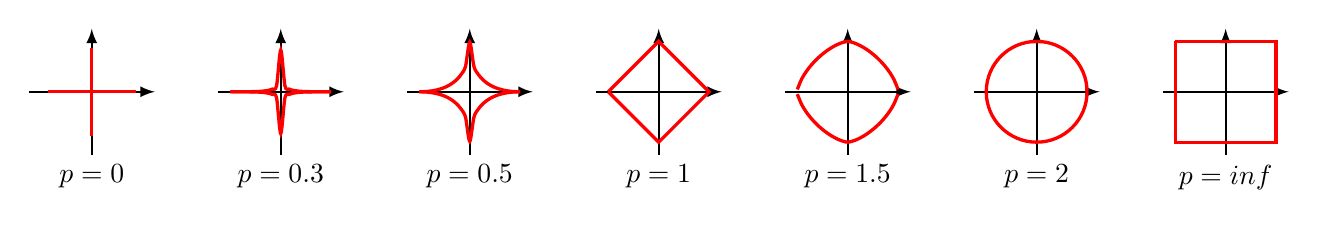
\begin{tikzpicture}[thick, >={latex}, scale=0.8]
		\draw[->] (0, 0) -- (2, 0);
		\draw[->] (1, -1) node[below] {$p=0$} -- (1, 1);
		\draw[red, very thick] (0.3, 0) -- (1.7, 0);
		\draw[red, very thick] (1, -0.7) -- (1, 0.7);
		
		\draw[->] (3, 0) -- (5, 0);
		\draw[->] (4, -1) node[below] {$p=0.3$} -- (4, 1);
		\draw[domain=-1:1, smooth, variable=\x, red, very thick]
			plot ({0.8*\x+4}, {0.8 * max(0.01, 1 - abs(\x)^0.3)^(1/0.3)});
			\draw[domain=-1:1, smooth, variable=\x, red, very thick]
			plot ({0.8*\x+4}, {-0.8 * max(0.01, 1 - abs(\x)^0.3)^(1/0.3)});
			
		\draw[->] (6, 0) -- (8, 0);
		\draw[->] (7, -1) node[below] {$p=0.5$} -- (7, 1);
		\draw[domain=-1:1, smooth, variable=\x, red, very thick]
			plot ({0.8*\x+7}, {0.8 * max(0.01, 1 - abs(\x)^0.5)^(1/0.5)});
		\draw[domain=-1:1, smooth, variable=\x, red, very thick]
			plot ({0.8*\x+7}, {-0.8 * max(0.01, 1 - abs(\x)^0.5)^(1/0.5)});
		
		\draw[->] (9, 0) -- (11, 0);
		\draw[->] (10, -1) node[below] {$p=1$} -- (10, 1);
		\draw[red, very thick] (9.2, 0) -- (10, 0.8) -- (10.8, 0) -- (10, -0.8) -- (9.2, 0);
		
		\draw[->] (12, 0) -- (14, 0);
		\draw[->] (13, -1) node[below] {$p=1.5$} -- (13, 1);
		\draw[domain=-1:1, smooth, variable=\x, red, very thick]
			plot ({0.8*\x+13}, {0.8 * max(0.01, 1 - abs(\x)^1.5)^(1/1.5)});
		\draw[domain=-1:1, smooth, variable=\x, red, very thick]
			plot ({0.8*\x+13}, {-0.8 * max(0.01, 1 - abs(\x)^1.5)^(1/1.5)});
		
		\draw[->] (15, 0) -- (17, 0);
		\draw[->] (16, -1) node[below] {$p=2$} -- (16, 1);
		\draw[red, very thick] (16, 0) circle (0.8);
		
		\draw[->] (18, 0) -- (20, 0);
		\draw[->] (19, -1) node[below] {$p=inf$} -- (19, 1);
		\draw[red, very thick] (18.2, 0.8) -- (19.8, 0.8) -- (19.8, -0.8) -- (18.2, -0.8) -- (18.2, 0.8);
	\end{tikzpicture}
\end{center}

La norme $l_2$ est utilisée pour réduire les risques d'overfitting en réduisant les plus grandes valeurs du modèle. La norme $l_1$, elle permet d'obtenir des modèles sparses, c'est à dire avec peu de features.

\exe
Considérons le problème suivant :
$$ \min_{\theta \in \R^d} \frac{1}{2} \theta^\trans \theta - \theta^\trans x + \lambda \| \theta \|_2^2 $$
Si $\lambda = 0$, alors :
$$ \dfrac{\partial \frac{1}{2} \theta^\trans \theta - \theta^\trans x}{\partial \theta_j} = 0 \Rightarrow \theta_j - x_j = 0 \Rightarrow \fbox{$\theta_j = x_j$} $$
Si $\lambda \neq 0$, alors :
$$ \dfrac{\partial \frac{1}{2} \theta^\trans \theta - \theta^\trans x  + \lambda \| \theta \|_2^2}{\partial \theta_j} = 0 \Rightarrow \theta_j - x_j +2\lambda \theta_j = 0 \Rightarrow \fbox{$\theta_j = \dfrac{x_j}{1 + 2\lambda}$} $$
\begin{center}
	\begin{tikzpicture}[>={latex}, thick]
	\draw[->] (-1, 0) -- (5, 0);
	\draw[->] (0, -1) -- (0, 3.5);
	\draw (3, 0) node {\tiny |} node[below] {3};
	\draw (0, 2) node {\tiny -} node[left] {2};
	\draw[fill] (3, 2) circle (0.05) node[below] {$x$};
	\draw[fill=greenTikz, fill opacity=0.5, very thick] (3, 2) circle (1.4^0.5);
	\draw[very thick] (3, 2) circle (1) circle (0.6^0.5) circle (0.2^0.5);
	\node[color=red] at (1, -0.6) {$\lambda = 0$};
	
	\draw[->] (7, 0) -- (13, 0);
	\draw[->] (8, -1) -- (8, 3.5);
	\draw (11, 0) node {\tiny |} node[below] {3};
	\draw (8, 2) node {\tiny -} node[left] {2};
	\draw[fill] (11, 2) circle (0.05) node[below] {$x$};
	\draw[fill=greenTikz, fill opacity=0.5, very thick] (9, 0.67) circle (0.47^0.5);
	\draw[very thick] (9, 0.67) circle (0.33^0.5) circle (0.2^0.5) circle (0.07^0.5);
	\node[color=red] at (9, -0.6) {$\lambda = 1$};
	\end{tikzpicture}
\end{center}

\exe
Maintenant on peut prendre la norme $l_1$ pour constater qu'elle engendre bien de la sparsité.
$$ \min_{\theta \in \R^d} \frac{1}{2} \theta^\trans \theta - \theta^\trans x + \lambda \| \theta \|_1 $$
Si $\lambda = 0$, on a vu que $\theta^* = x$. \\
En revanche si $\lambda > 0$, on considère la dérivée partielle à $\theta_j = 0^+$, et à $\theta_j = 0^-$ :
$$ g_+^j = \lambda - x_j \qquad g_-^j = - \lambda - x_j $$
Or $\theta_j^* = 0$ si et seulement si $g_+^j \geqslant 0$ et $g_-^j \leqslant 0$. C'est à dire si $x_j \geqslant \lambda$ et $x_j \leqslant -\lambda$. \\
Donc si $|x_j| \leqslant \lambda$ alors $\theta_j^* = 0$.
\begin{center}
	\begin{tikzpicture}[>={latex}, thick, scale=0.8]
	\draw[->] (-1, 0) -- (5, 0);
	\draw[->] (0, -1) -- (0, 3.5);
	\draw (3, 0) node {\tiny |} node[below] {3};
	\draw (0, 2) node {\tiny -} node[left] {2};
	\node[color=red] at (1, -0.6) {$\lambda = 0$};
	\draw[fill] (3, 2) circle (0.05) node[below] {$x$};
	\draw[fill=greenTikz, fill opacity=0.5, very thick] (3, 2) circle (5^0.5);
	\draw[very thick] (3, 2) circle (3^0.5) circle (1);
	
	\draw[->] (7, 0) -- (13, 0);
	\draw[->] (8, -1) -- (8, 3.5);
	\draw (11, 0) node {\tiny |} node[below] {3};
	\draw (8, 2) node {\tiny -} node[left] {2};
	\draw[fill] (11, 2) circle (0.05) node[below] {$x$};
	\draw[fill, red] (9, 0) circle (0.05) node[above] {$\theta^*$};
	\node[color=red] at (12.4, 3) {$\lambda = 2$};
	\node[color=red] at (12.4, 2.5) {$\theta^*$ est sparse};
	\draw[very thick, fill=greenTikz, fill opacity=0.5] (11.24, 0) arc (0:116.6:2.24);
	\draw[very thick, fill=greenTikz, fill opacity=0.5] (8, 2) arc (158:180:5.39);
	\draw[very thick, fill=greenTikz, fill opacity=0.5] (7.61, 0) arc (217:222.4:6.71);
	\draw[very thick, fill=greenTikz, fill opacity=0.5] (8, -0.47) arc (257.4:299.1:4.58);
	\draw[very thick] (10, 0) arc(0:180:1);
	\draw[very thick] (8, 0) arc(-104:-76:4.12);
	\draw[very thick] (10.73, 0) arc(0:125:3^0.5);
	\draw[very thick] (7.8, 0) arc(180:164:27^0.5);
	\draw[very thick] (7.8, 0) arc(217.6:220.5:43^0.5);
	\draw[very thick] (10.73, 0) arc(-66.6:-103:19^0.5);
	\fill[greenTikz, opacity=0.5] (11.24, 0) -- (8, 2) -- (7.61, 0) -- (8, -0.47);
	\end{tikzpicture}
\end{center}

\paragraph{Supprimer des groupes de features}
Voici des normes qui permettent de supprimer les features en groupe :
\begin{center}
	\includegraphics[scale=0.5]{group_sparse.png}
\end{center}
On considère $\{ \mathcal{G}_{k = 1}^K \}$ une partition de $\{ 1, \dots, d \}$. On peur alors définir les normes suivantes :
$$ \| \theta \|_{group} = \sum_{g \in \mathcal{G}} \left( \sum_{j \in g} \theta_j^2 \right)^{\frac{1}{2}} $$
$$ \| \theta \|_{coop} = \sum_{g \in \mathcal{G}} \left[ \left( \sum_{j \in g} [\theta_j]_+^2 \right)^{\frac{1}{2}} + \left( \sum_{j \in g} [\theta_j]_-^2 \right)^{\frac{1}{2}} \right] $$


\subs{Contrepartie Biais/Variance}

\subs{Bornes de généralisation}

\subs{Choix du modèle}